\chapter{Symulacje}
W ramach pracy został przeprowadzony zestaw scenariuszy symulacyjnych. Każdy z zaimplementowanych protokołów został przetestowany z przygotowanymi zestawami parametrów wejściowych.
Do tych parametrów należą:
\paragraph{Dystrybucja węzłów sieci}
Symulacje zostały przeprowadzone dla dwóch sposobów dystrybucji węzłów: zgodnej z rozkładem normalnym oraz zgodnej z rozkładem jednorodnym.

Dla rozkładu normalnego średnia współrzędnej wynosiła 400m, a jej odchylenie standardowe 100m.

\begin{figure}[!htbp]
	\begin{center}
		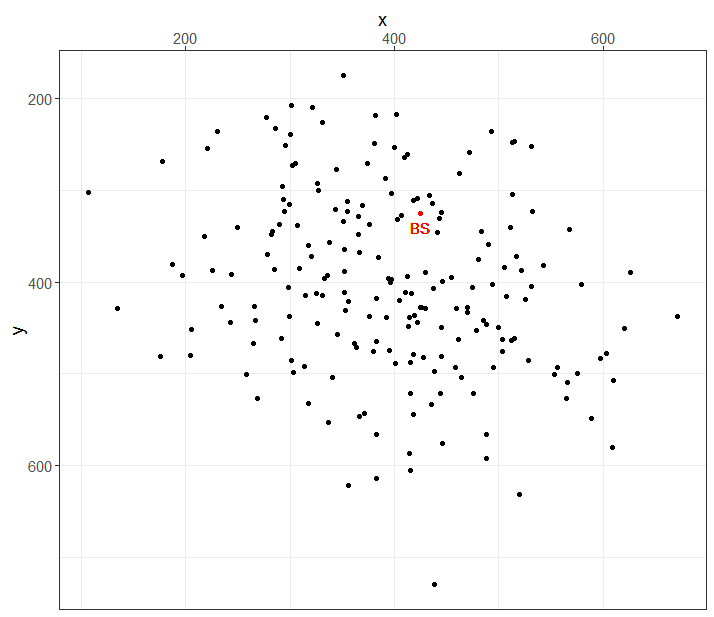
\includegraphics[scale=0.35]{\ImgPath/charts/normal_distribution.png}
	\end{center}
	\caption{Przykładowa dystrybucja węzłów sieci zgodna z rozkładem normalnym}
\end{figure}

Z rozkładem jednorodnym węzły zostały rozłożone na obszarze o kształcie prostokąta o wymiarach 450m na 550m.

\begin{figure}[!htbp]
	\begin{center}
		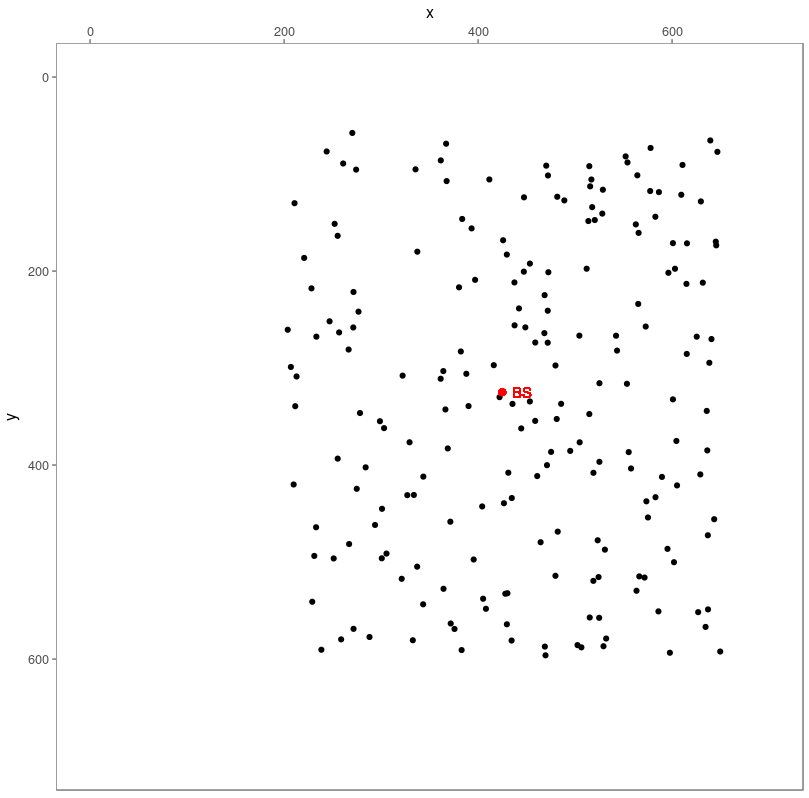
\includegraphics[scale=0.35]{\ImgPath/charts/uniform_distribution.png}
	\end{center}
	\caption{Przykładowa dystrybucja węzłów sieci zgodna z rozkładem jednorodnym}
\end{figure}

\paragraph{Liczba węzłów sieci}
Symulacje przeprowadzono dla sieci składającej się z dwudziestu oraz dwustu czujników.
\paragraph{Rozmiar pakietu z danymi}
Symulacje przeprowadzono dla rozmiarów pakietów 5B, 50B, 500B, 5000B.
\paragraph{Częstotliwość generowania nowych danych}
Symulacje przeprowadzono dla okresów generowania danych wynoszących: 5s, 10s, 15s, 20s.
\paragraph{Początkowa wartość energii elektrycznej w węźle}
Jako początkową wartość dla czujnika przyjęto 5J, co odpowiada baterii R6 (AA) w skali 1:1000.
%uzasadnić na krzywej zużycia baterii

Dodatkowo dla protokołów z rodziny LEACH zdefiniowane zostały parametry:
\paragraph{Procent lokalnych węzłów bazowych w sieci}
\paragraph{Długość rundy}

W celu zniwelowania wpływu losowego rozmieszczenia węzłów na długość działania sieci, dla każdego pojedynczego zestawu parametrów wykonano 5 przebiegów symulacji z różnym ziarnem. Wyniki tych przebiegów zostały uśrednione.

Dla każdej symulacji zostały również zdefiniowane stałe warunki środowiskowe:
\begin{itemize}
	\item Przestrzeń - idealnie płaski teren bez żadnych przeszkód.
	\item Prędkość propagacji fali - założono model propagacji fali ze stałą prędkością. Oznacza to, że czas propagacji jest proporcjonalny do przebytej odległości zdeterminowanej przez stały parametr prędkości.
	\item Tłumienie trasy radiowej - założono model Breakpoint path loss.
	\item Szum tła - założono szum izotropowy o mocy -96.616dBm.
	\item Do reprezentacji sygnału analogowego wykorzystany został model skalarny - opisuje on sygnał za pomocą jego mocy skalarnej, szerokości pasma oraz częstotliwości fali nośnej.
\end{itemize}